\section{Sistema Propuesto}
Esta sección se enfoca en la descripción de la solución propuesta, se identifican las actividades que fueron realizadas durante la estadía, así como una descripción de los procesos que se llevaron a cabo para la implementación del sistema. A continuación, la figura \ref{fig:porcentaje-actividades} muestra las actividades que se llevaron a cabo durante la estadía y su porcentaje de tiempo dedicado.

\begin{figure}[H]
    \centering
    \begin{tikzpicture}
        \pie[
            color = {
                yellow!90!black, 
                green!60!black, 
                blue!60, 
                red!70,
                gray!70,
                teal!20},
            text = legend
        ]
        {10/Análisis de Requerimientos,
            10/Diseño de la Arquitectura del Sistema,
            10/Diseño de la Base de Datos,
            25/Diseño de la Interfaz de Usuario,
            40/Desarrollo del Backend,
            5/Despliegue del Software}
    \end{tikzpicture}
    \caption{Porcentaje de tiempo dedicado a las actividades realizadas durante la estadía}
\label{fig:porcentaje-actividades}
\end{figure}

También se muestra el diagrama de Gantt en la figura \ref{fig:gantt} que muestra las actividades realizadas durante la estadía y su duración en semanas.


\begin{figure}[H]
    \centering
    \begin{ganttchart}[
        hgrid,
        vgrid,
        x unit=0.75cm,
        y unit title=0.6cm,
        y unit chart=0.6cm,
        title label font=\footnotesize,
        title height=1,
        bar label font=\footnotesize,
        bar height=0.5,
        group label font=\footnotesize,
        milestone label font=\footnotesize,
        milestone height=0.5,
        bar incomplete/.append style={fill=red!50}
    ]{1}{16}
    \gantttitle{Mayo}{4}
    \gantttitle{Junio}{4}
    \gantttitle{Julio}{4}
    \gantttitle{Agosto}{4} \\
    
    \ganttgroup{Análisis de Requerimientos}{1}{2} \\
    \ganttgroup{Diseño de la Arquitectura}{2}{3} \\
    \ganttgroup{Diseño de la Base de Datos}{3}{4} \\
    \ganttgroup{Diseño de la Interfaz de Usuario}{4}{8} \\
    \ganttgroup{Desarrollo del Backend}{5}{12} \\
    \ganttgroup{Pruebas y Depuración}{10}{14} \\
    \ganttgroup{Despliegue del Software}{14}{16} \\
    \end{ganttchart}
    \caption{Diagrama de Gantt de las actividades realizadas durante la estadía}
    \label{fig:gantt}
\end{figure}

\subsection{Análisis de Requerimientos}
El primer paso para el desarrollo de este proyecto fue la identificación de los requerimientos del sistema. Para ello, se realizaron diversas entrevistas con el doctor Marco Aurelio Nuño Maganda, quien es el principal interesado en el desarrollo de este proyecto. Se identificaron los requerimientos funcionales y no funcionales del sistema, así como los casos de uso que se llevarán a cabo en el sistema. A continuación, se describen los requerimientos del sistema. 

\subsubsection{Requerimientos Funcionales}
Los requerimientos funcionales del sistema, derivados de las entrevistas con el interesado, son los siguientes:

\begin{enumerate}
    \item \textbf{Gestión de Usuarios}:
    \begin{itemize}
        \item Crear nuevos usuarios.
        \item Cada usuario debe tener un perfil personal.
        \item Cada usuario debe poder crear y gestionar sus coautores (añadir, editar, eliminar).
    \end{itemize}

    \item \textbf{Gestión de Plantillas LaTeX}:
    \begin{itemize}
        \item Subir plantillas LaTeX personalizadas.
        \item Ver y previsualizar las plantillas.
        \item Compilar una plantilla básica sin necesidad de subirla.
        \item Guardar, editar y eliminar plantillas LaTeX.
    \end{itemize}

    \item \textbf{Creación y Edición de Artículos}:
    \begin{itemize}
        \item Crear nuevos artículos.
        \item Editar detalles del artículo.
        \item Agregar títulos, texto simple, imágenes, código LaTeX embebido, listas y referencias a los artículos.
        \item Compilar el contenido del artículo en las plantillas cargadas.
        \item Agregar referencias en formato .bib.
        \item Descargar el PDF generado del artículo.
        \item Descargar el archivo ZIP del artículo generado con la plantilla seleccionada.
    \end{itemize}

    \item \textbf{Gestión de Artículos}:
    \begin{itemize}
        \item Ver los artículos creados por el usuario.
        \item Editar y eliminar artículos creados por el usuario.
        \item Añdir y borrar coautores de los artículos.
    \end{itemize}

    \item \textbf{Seguridad y Sesiones}:
    \begin{itemize}
        \item Manejar sesiones de usuario.
        \item Cambiar contraseña.
        \item Implementar autenticación de dos factores.
        \item Recuperar contraseña.
        \item Eliminar cuenta de usuario.
    \end{itemize}
\end{enumerate}

\subsubsection{Requerimientos No Funcionales}
Los requerimientos no funcionales del sistema incluyen:

\begin{enumerate}
    \item \textbf{Rendimiento}:
    \begin{itemize}
        \item El sistema debe ser capaz de manejar múltiples solicitudes simultáneamente sin degradar el rendimiento.
        \item La compilación de plantillas y la generación de PDFs debe ser rápida y eficiente.
    \end{itemize}

    \item \textbf{Usabilidad}:
    \begin{itemize}
        \item La interfaz de usuario debe ser intuitiva y fácil de navegar.
        \item Los usuarios deben poder realizar todas las operaciones con un mínimo de pasos y esfuerzo.
    \end{itemize}

    \item \textbf{Escalabilidad}:
    \begin{itemize}
        \item El sistema debe ser capaz de escalar para soportar un creciente número de usuarios y datos.
    \end{itemize}

    \item \textbf{Seguridad}:
    \begin{itemize}
        \item Los datos de los usuarios deben estar protegidos contra accesos no autorizados.
        \item El sistema debe cumplir con las normativas de seguridad y privacidad de datos vigentes.
    \end{itemize}

    \item \textbf{Mantenibilidad}:
    \begin{itemize}
        \item El sistema debe estar diseñado de manera que sea fácil de mantener y actualizar.
        \item El código debe estar bien documentado y seguir buenas prácticas de desarrollo.
    \end{itemize}
\end{enumerate}


\subsection{Arquitectura del Sistema}
La arquitectura del sistema propuesto se basa en una arquitectura de tres capas, que consta de una capa de presentación, una capa de lógica de negocio y una capa de acceso a datos. Esta estructura fue seleccionada por su capacidad para organizar el código de manera modular, facilitando la mantenibilidad y escalabilidad del sistema. La figura \ref{fig:arquitectura-sistema} muestra la arquitectura del sistema propuesto.

\begin{figure}[H]
    \centering
    \begin{tikzpicture}[node distance=2cm, auto]
        % Styles
        \tikzstyle{controller} = [rectangle, rounded corners, minimum width=2cm, minimum height=1cm,text centered, draw=black, fill=blue!20]
        \tikzstyle{model} = [rectangle, rounded corners, minimum width=2cm, minimum height=1cm,text centered, draw=black, fill=green!20]
        \tikzstyle{view} = [rectangle, rounded corners, minimum width=2cm, minimum height=1cm,text centered, draw=black, fill=red!20]

        % Nodes
        \node[controller] (controller) {Controlador};
        \node[model, above right=of controller] (model) {Modelo};
        \node[view, below right=of controller] (view) {Vista};
        \node[right=1cm of model] (database) {Base de Datos};

        % Arrows
        \draw[-{Latex[length=3mm]}, thick, dashed] (model) to [bend left=15] node[midway, above] {} (view);

        \draw[-{Latex[length=3mm]}, thick] (view) to [bend left=15] node[midway, below] {} (model);

         \draw[-{Latex[length=3mm]}, thick, dashed] (view) to [bend left=15] node[midway, below] {} (controller);
         
         \draw[-{Latex[length=3mm]}, thick, dashed] (controller) to [bend left=15] node[midway, below] {} (view);
        
        \draw[-{Latex[length=3mm]}, thick] (controller) to [bend left=15] node[midway, below] {} (model);
                
        \draw[-{Latex[length=3mm]}, thick] (model) to [bend right=45] node[midway, left] {} (database);

    \end{tikzpicture}
    \caption{Arquitectura MVC del proyecto}
    \label{fig:arquitectura-sistema}
\end{figure}

\subsubsection{Capa de Presentación}
La capa de presentación o de vistas consta de la interfaz de usuario del sistema. Se decidió utilizar el framework Laravel debido a su potente motor de plantillas Blade, el cual permite crear interfaces web funcionales de manera eficiente. Esta capa es responsable de recibir las solicitudes de los usuarios y de mostrarles la información procesada por la capa de lógica de negocio. La elección de este facilita la implementación de una interfaz de usuario coherente y responsiva, lo cual es esencial para mejorar la experiencia del usuario final y garantizar la usabilidad del sistema en distintos dispositivos y navegadores. Se tomó el cuenta que la capa de presentación debe ser fácil de usar y navegar pero también debe ser flexible y escalable para futuras actualizaciones y mejoras, es por ello que en esta capa se implementaron compomentes reutilizables y modulares que permiten una fácil extensión del sistema.

\subsubsection{Capa de Lógica de Negocio}
La capa de lógica de negocio es el núcleo del sistema y es donde se implementan todas las reglas y procesos detrás de la aplicación. Al emplear Laravel, se aprovechan sus características, como lo son los controladores y middleware, para gestionar las operaciones del sistema de manera eficiente y segura. Esta capa maneja la creación, edición y eliminación de usuarios, plantillas y artículos, manejando las interacciones entre la capa de presentación y la capa de acceso a datos. La modularidad que ofrece en esta capa aseguran un desarrollo más ordenado y facilitan futuras ampliaciones del sistema, permitiendo una fácil integración de nuevas funcionalidades y la corrección de errores de manera rápida y efectiva debido a la modularidad de los componentes.

\subsubsection{Capa de Acceso a Datos}
La capa de acceso a datos se encarga de la persistencia y recuperación de la información almacenada. Se utiliza Eloquent ORM (Object-Relational Mapping), que proporciona una lógica intuitiva para interactuar con la base de datos. Esta herramienta permite gestionar las relaciones entre las distintas entidades del sistema de manera eficiente, garantizando un acceso rápido y seguro a los datos. La elección de Eloquent ORM se basa en su capacidad para simplificar la interacción con la base de datos, reduciendo significativamente el esfuerzo de codificación y minimizando los errores potenciales. La elección de Eloquent ORM nos permite facilitar las operaciones a la hora de crear y gestionar los datos de los usuarios como lo son sus plantillas y artículos, además de permitir una fácil integración con la capa de lógica de negocio y la capa de presentación.

\subsubsection{Justificación de la Arquitectura Seleccionada}
La arquitectura de tres capas fue seleccionada para este proyecto debido a sus múltiples ventajas en términos de organización, mantenibilidad y escalabilidad del sistema. La separación de responsabilidades en distintas capas permite que cada una se enfoque en un aspecto específico del sistema, facilitando así su desarrollo y mantenimiento. 

1. Modularidad: La arquitectura de tres capas permite un desarrollo modular, donde cada componente puede ser desarrollado, probado y mantenido de manera independiente. Esto mejora la eficiencia del equipo de desarrollo y reduce el tiempo de implementación de nuevas funcionalidades.

2. Escalabilidad: Esta arquitectura facilita la escalabilidad del sistema. Si el número de usuarios o la cantidad de datos crece, es posible escalar cada capa de manera independiente, optimizando recursos y costos.

3. Mantenibilidad: La clara separación de responsabilidades facilita la localización y corrección de errores, así como la implementación de mejoras. El uso de Laravel contribuye significativamente a este aspecto, gracias a su estructura ordenada y su extensa documentación.

4. Seguridad: Al contar con una capa de acceso a datos bien definida, es más sencillo implementar y gestionar las medidas de seguridad necesarias para proteger la información del sistema. El framework proporciona múltiples mecanismos de seguridad integrados, que se ajustan a las necesidades del proyecto.


\subsection{Diagrama de Contexto}
Para visualizar las interacciones entre los actores y el sistema, se elaboró un diagrama de contexto que muestra las operaciones que pueden realizar los usuarios y el sistema. La figura \ref{fig:diagrama-contexto} muestra el diagrama de contexto del sistema de gestión de artículos, donde se identifican los actores principales y las interacciones entre ellos.

\begin{figure}[H]
    \centering
    \begin{tikzpicture}[node distance=2cm, auto]
        % Styles
        \tikzstyle{system} = [rectangle, rounded corners, minimum width=4cm, minimum height=1cm,text centered, draw=black, fill=blue!20]
        \tikzstyle{external} = [rectangle, minimum width=3cm, minimum height=1cm, text centered, draw=black, fill=green!20]

        % Nodes
        \node[system] (system) {Sistema de Gestión de Artículos};
        \node[external, above=of system] (user) {Usuario};
        \node[external, below=of system] (db) {Base de Datos};

        % Arrows
        \draw[-Stealth, thick] (user) -- (system) node[midway, left] {Interacción con UI};
        \draw[-Stealth, thick] (system) -- (db) node[midway, right] {Acceso a Datos};
        \draw[-Stealth, thick] (db) -- (system) node[midway, right] {};

    \end{tikzpicture}
    \caption{Diagrama de Contexto del Sistema de Gestión de Artículos}
    \label{fig:diagrama-contexto}
\end{figure}

\subsection{Diagrama de Casos de Uso}
Para identificar las funcionalidades del sistema y las interacciones entre los actores y el sistema, se elaboró un diagrama de casos de uso. La figura \ref{fig:casos-uso} muestra el diagrama de casos de uso del sistema de gestión de artículos, donde se identifica al usuario como el actor principal y las operaciones que puede realizar en el sistema. 

% IMAGENES/caso-uso.png escalar imagen a 0.5
\begin{figure}[H]
    \centering
    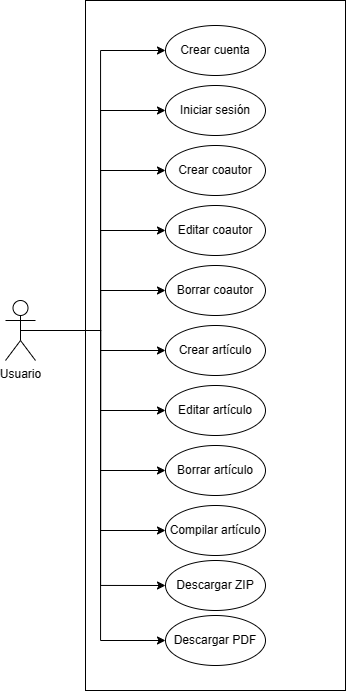
\includegraphics[scale=0.5]{IMAGENES/caso-uso.png}
    \caption{Diagrama de Casos de Uso del Sistema de Gestión de Artículos}
    \label{fig:casos-uso}
\end{figure}

Para un mejor entendimiento de los casos de uso, se decidió hacer el modelado de los requisitos obtenidos para conocer todas las actividades, flujos de información y manejo de errores de cada una de las acciones que hará el usuario.

En el cuadro \ref{tab:caso-uso-crear-cuenta} se muestra el caso de uso para la creación de una cuenta de usuario en el sistema. En este caso, el usuario debe ingresar su nombre, datos de autor, correo electrónico y contraseña para crear una cuenta. Si los datos son válidos, el sistema le permitirá crear la cuenta y acceder a su perfil. En caso de que los datos sean incorrectos o ya exista una cuenta con el mismo correo electrónico, el sistema mostrará un mensaje de error y le dará la opción de intentarlo nuevamente.

\begin{table}[H]
    \centering
        \begin{tabular}{|p{0.5cm}|p{3.5cm}|p{10cm}|}
        \hline
        \textbf{ID} & \textbf{Caso de Uso} & \textbf{Crear Cuenta} \\
        \hline
        1 & \textbf{Descripción} & El usuario crea una cuenta en el sistema. \\
        \hline
        2 & \textbf{Actores} & Usuario. \\
        \hline
        3 & \textbf{Precondiciones} & El usuario no debe tener una cuenta en el sistema. \\
        \hline
        4 & \textbf{Flujo Principal} & 
        \begin{enumerate}
            \item El usuario ingresa su nombre, datos de autor, correo electrónico y contraseña.
            \item El sistema verifica los datos ingresados.
            \item El sistema crea la cuenta del usuario.
        \end{enumerate} \\
        \hline
        5 & \textbf{Flujo Alternativo} & 
        \begin{enumerate}
            \item El sistema muestra un mensaje de error si los datos son incorrectos o ya existe una cuenta con el mismo correo electrónico.
            \item El usuario puede intentarlo nuevamente.
        \end{enumerate} \\
        \hline
        6 & \textbf{Postcondiciones} & El usuario crea una cuenta en el sistema. \\
        \hline
    \end{tabular}
    \caption{Caso de Uso: Crear Cuenta}
    \label{tab:caso-uso-crear-cuenta}
\end{table}

En el cuadro \ref{tab:caso-uso-iniciar-sesion} se muestra el caso de uso para el inicio de sesión de un usuario en el sistema. En este caso, el usuario debe ingresar su correo electrónico y contraseña para acceder al sistema. Si los datos son correctos, el sistema le permitirá acceder a su perfil. En caso de que los datos sean incorrectos, el sistema mostrará un mensaje de error y le dará la opción de intentarlo nuevamente.

\begin{table}[H]
    \centering
        \begin{tabular}{|p{0.5cm}|p{3.5cm}|p{10cm}|}
        \hline
        \textbf{ID} & \textbf{Caso de Uso} & \textbf{Iniciar Sesión} \\
        \hline
        1 & \textbf{Descripción} & El usuario inicia sesión en el sistema. \\
        \hline
        2 & \textbf{Actores} & Usuario. \\
        \hline
        3 & \textbf{Precondiciones} & El usuario debe tener una cuenta en el sistema. \\
        \hline
        4 & \textbf{Flujo Principal} & 
        \begin{enumerate}
            \item El usuario ingresa su correo electrónico y contraseña.
            \item El sistema verifica los datos ingresados.
            \item El sistema muestra el perfil del usuario.
        \end{enumerate} \\
        \hline
        5 & \textbf{Flujo Alternativo} & 
        \begin{enumerate}
            \item El sistema muestra un mensaje de error si los datos son incorrectos.
            \item El usuario puede intentarlo nuevamente.
        \end{enumerate} \\
        \hline
        6 & \textbf{Postcondiciones} & El usuario accede a su perfil en el sistema. \\
        \hline
    \end{tabular}
    \caption{Caso de Uso: Iniciar Sesión}
    \label{tab:caso-uso-iniciar-sesion}
\end{table}

En el cuadro \ref{tab:caso-uso-crear-articulo} se muestra el caso de uso para la creación de un artículo en el sistema. En este caso, el usuario debe ingresar los datos del artículo, como el título, el contenido y las referencias. El sistema le permitirá guardar el artículo y compilarlo en una plantilla LaTeX. Si el artículo se guarda correctamente, el sistema mostrará un mensaje de confirmación y le dará la opción de descargar el PDF generado.

\begin{table}[H]
    \centering
        \begin{tabular}{|p{0.5cm}|p{3.5cm}|p{10cm}|}
        \hline
        \textbf{ID} & \textbf{Caso de Uso} & \textbf{Crear Artículo} \\
        \hline
        1 & \textbf{Descripción} & El usuario crea un artículo en el sistema. \\
        \hline
        2 & \textbf{Actores} & Usuario. \\
        \hline
        3 & \textbf{Precondiciones} & El usuario debe haber iniciado sesión en el sistema. \\
        \hline
        4 & \textbf{Flujo Principal} & 
        \begin{enumerate}
            \item El usuario ingresa el título, contenido y referencias del artículo.
            \item El sistema guarda el artículo.
            \item El sistema compila el artículo en una plantilla LaTeX.
            \item El sistema muestra un mensaje de confirmación.
        \end{enumerate} \\
        \hline
        5 & \textbf{Flujo Alternativo} & 
        \begin{enumerate}
            \item El sistema muestra un mensaje de error si los datos son incorrectos.
            \item El usuario puede intentarlo nuevamente.
        \end{enumerate} \\
        \hline
        6 & \textbf{Postcondiciones} & El usuario crea un artículo en el sistema. \\
        \hline
    \end{tabular}
    \caption{Caso de Uso: Crear Artículo}
    \label{tab:caso-uso-crear-articulo}

\end{table}

En el cuadro \ref{tab:caso-uso-editar-articulo} se muestra el caso de uso para la edición de un artículo en el sistema. En este caso, el usuario puede editar los datos del artículo, como el título, el contenido, los coautores y las referencias. El sistema le permitirá guardar los cambios y compilar el artículo en una plantilla LaTeX. Si los cambios se guardan correctamente, el sistema mostrará un mensaje de confirmación y le dará la opción de descargar el PDF generado.

\begin{table}[H]
    \centering
        \begin{tabular}{|p{0.5cm}|p{3.5cm}|p{10cm}|}
        \hline
        \textbf{ID} & \textbf{Caso de Uso} & \textbf{Editar Artículo} \\
        \hline
        1 & \textbf{Descripción} & El usuario edita un artículo en el sistema. \\
        \hline
        2 & \textbf{Actores} & Usuario. \\
        \hline
        3 & \textbf{Precondiciones} & El usuario debe haber iniciado sesión en el sistema y tener un artículo creado. \\
        \hline
        4 & \textbf{Flujo Principal} & 
        \begin{enumerate}
            \item El usuario selecciona el artículo a editar.
            \item El usuario edita los datos del artículo.
            \item El sistema guarda los cambios.
            \item El sistema compila el artículo en una plantilla LaTeX.
            \item El sistema muestra un mensaje de confirmación.
        \end{enumerate} \\
        \hline
        5 & \textbf{Flujo Alternativo} & 
        \begin{enumerate}
            \item El sistema muestra un mensaje de error si los datos son incorrectos.
            \item El usuario puede intentarlo nuevamente.
        \end{enumerate} \\
        \hline
        6 & \textbf{Postcondiciones} & El usuario edita un artículo en el sistema. \\
        \hline
    \end{tabular}
    \caption{Caso de Uso: Editar Artículo}
    \label{tab:caso-uso-editar-articulo}
\end{table}



En el cuadro \ref{tab:caso-uso-borrar-articulo} se muestra el caso de uso para la eliminación de un artículo en el sistema. En este caso, el usuario puede seleccionar un artículo y borrarlo del sistema. El sistema le mostrará un mensaje de confirmación y le dará la opción de borrar el artículo definitivamente.

\begin{table}[H]
    \centering
        \begin{tabular}{|p{0.5cm}|p{3.5cm}|p{10cm}|}
        \hline
        \textbf{ID} & \textbf{Caso de Uso} & \textbf{Borrar Artículo} \\
        \hline
        1 & \textbf{Descripción} & El usuario borra un artículo en el sistema. \\
        \hline
        2 & \textbf{Actores} & Usuario. \\
        \hline
        3 & \textbf{Precondiciones} & El usuario debe haber iniciado sesión en el sistema y tener un artículo creado. \\
        \hline
        4 & \textbf{Flujo Principal} & 
        \begin{enumerate}
            \item El usuario selecciona el artículo a borrar.
            \item El sistema muestra un mensaje de confirmación.
            \item El usuario confirma la eliminación del artículo.
        \end{enumerate} \\
        \hline
        5 & \textbf{Flujo Alternativo} & 
        \begin{enumerate}
            \item El usuario cancela la eliminación del artículo.
            \item El sistema muestra un mensaje de confirmación.
        \end{enumerate} \\
        \hline
        6 & \textbf{Postcondiciones} & El usuario borra un artículo en el sistema. \\
        \hline
    \end{tabular}
    \caption{Caso de Uso: Borrar Artículo}
    \label{tab:caso-uso-borrar-articulo}
\end{table}

En el cuadro \ref{tab:caso-uso-crear-coautor} se muestra el caso de uso para la creación de un coautor en el sistema. En este caso, el usuario puede agregar un coator a la lista de coautores con los que ha trabajado en un artículo. El sistema le permitirá guardar los cambios y mostrará un mensaje de confirmación si la operación es exitosa.

\begin{table}[H]
    \centering
        \begin{tabular}{|p{0.5cm}|p{3.5cm}|p{10cm}|}
        \hline
        \textbf{ID} & \textbf{Caso de Uso} & \textbf{Crear Coautor} \\
        \hline
        1 & \textbf{Descripción} & El usuario crea un coautor en el sistema. \\
        \hline
        2 & \textbf{Actores} & Usuario. \\
        \hline
        3 & \textbf{Precondiciones} & El usuario debe haber iniciado sesión en el sistema y tener un artículo creado. \\
        \hline
        4 & \textbf{Flujo Principal} & 
        \begin{enumerate}
            \item El usuario selecciona el artículo al que desea agregar un coautor.
            \item El usuario agrega el coautor a la lista de coautores.
            \item El sistema guarda los cambios.
            \item El sistema muestra un mensaje de confirmación.
        \end{enumerate} \\
        \hline
        5 & \textbf{Flujo Alternativo} & 
        \begin{enumerate}
            \item El sistema muestra un mensaje de error si los datos son incorrectos.
            \item El usuario puede intentarlo nuevamente.
        \end{enumerate} \\
        \hline
        6 & \textbf{Postcondiciones} & El usuario crea un coautor en el sistema. \\
        \hline
    \end{tabular}
    \caption{Caso de Uso: Crear Coautor}
    \label{tab:caso-uso-crear-coautor}

\end{table}

En el cuadro \ref{tab:caso-uso-editar-coautor} se muestra el caso de uso para la edición de un coautor en el sistema. En este caso, el usuario puede seleccionar un coautor y editar sus datos. El sistema le permitirá guardar los cambios y mostrará un mensaje de confirmación si la operación es exitosa.

\begin{table}[H]
    \centering
        \begin{tabular}{|p{0.5cm}|p{3.5cm}|p{10cm}|}
        \hline
        \textbf{ID} & \textbf{Caso de Uso} & \textbf{Editar Coautor} \\
        \hline
        1 & \textbf{Descripción} & El usuario edita un coautor en el sistema. \\
        \hline
        2 & \textbf{Actores} & Usuario. \\
        \hline
        3 & \textbf{Precondiciones} & El usuario debe haber iniciado sesión en el sistema y tener un coautor creado. \\
        \hline
        4 & \textbf{Flujo Principal} & 
        \begin{enumerate}
            \item El usuario selecciona el coautor a editar.
            \item El usuario edita los datos del coautor.
            \item El sistema guarda los cambios.
            \item El sistema muestra un mensaje de confirmación.
        \end{enumerate} \\
        \hline
        5 & \textbf{Flujo Alternativo} & 
        \begin{enumerate}
            \item El sistema muestra un mensaje de error si los datos son incorrectos.
            \item El usuario puede intentarlo nuevamente.
        \end{enumerate} \\
        \hline
        6 & \textbf{Postcondiciones} & El usuario edita un coautor en el sistema. \\
        \hline
    \end{tabular}
    \caption{Caso de Uso: Editar Coautor}
    \label{tab:caso-uso-editar-coautor}

\end{table}

En el cuadro \ref{tab:caso-uso-borrar-coautor} se muestra el caso de uso para la eliminación de un coautor en el sistema. En este caso, el usuario puede seleccionar un coautor y borrarlo del sistema. El sistema le mostrará un mensaje de confirmación y le dará la opción de borrar el coautor definitivamente.

\begin{table}[H]
    \centering
        \begin{tabular}{|p{0.5cm}|p{3.5cm}|p{10cm}|}
        \hline
        \textbf{ID} & \textbf{Caso de Uso} & \textbf{Borrar Coautor} \\
        \hline
        1 & \textbf{Descripción} & El usuario borra un coautor en el sistema. \\
        \hline
        2 & \textbf{Actores} & Usuario. \\
        \hline
        3 & \textbf{Precondiciones} & El usuario debe haber iniciado sesión en el sistema y tener un coautor creado. \\
        \hline
        4 & \textbf{Flujo Principal} & 
        \begin{enumerate}
            \item El usuario selecciona el coautor a borrar.
            \item El sistema muestra un mensaje de confirmación.
            \item El usuario confirma la eliminación del coautor.
        \end{enumerate} \\
        \hline
        5 & \textbf{Flujo Alternativo} & 
        \begin{enumerate}
            \item El usuario cancela la eliminación del coautor.
            \item El sistema muestra un mensaje de confirmación.
        \end{enumerate} \\
        \hline
        6 & \textbf{Postcondiciones} & El usuario borra un coautor en el sistema. \\
        \hline
    \end{tabular}
    \caption{Caso de Uso: Borrar Coautor}
    \label{tab:caso-uso-borrar-coautor}
\end{table}

En el cuadro \ref{tab:caso-uso-subir-plantilla} se muestra el caso de uso para la subida de una plantilla LaTeX en formato .zip al sistema. En este caso, el usuario debe seleccionar un archivo .zip que contenga la plantilla LaTeX y subirlo al sistema. El sistema le permitirá guardar la plantilla y mostrará un mensaje de confirmación si la subida es exitosa.

\begin{table}[H]
    \centering
        \begin{tabular}{|p{0.5cm}|p{3.5cm}|p{10cm}|}
        \hline
        \textbf{ID} & \textbf{Caso de Uso} & \textbf{Subir Plantilla LaTeX} \\
        \hline
        1 & \textbf{Descripción} & El usuario sube una plantilla LaTeX al sistema. \\
        \hline
        2 & \textbf{Actores} & Usuario. \\
        \hline
        3 & \textbf{Precondiciones} & El usuario debe haber iniciado sesión en el sistema. \\
        \hline
        4 & \textbf{Flujo Principal} & 
        \begin{enumerate}
            \item El usuario selecciona un archivo .zip que contenga la plantilla LaTeX.
            \item El sistema guarda la plantilla en la base de datos.
            \item El sistema muestra un mensaje de confirmación.
        \end{enumerate} \\
        \hline
        5 & \textbf{Flujo Alternativo} & 
        \begin{enumerate}
            \item El sistema muestra un mensaje de error si el archivo no es válido.
            \item El usuario puede intentarlo nuevamente.
        \end{enumerate} \\
        \hline
        6 & \textbf{Postcondiciones} & El usuario sube una plantilla LaTeX al sistema. \\
        \hline
    \end{tabular}
    \caption{Caso de Uso: Subir Plantilla LaTeX}
\label{tab:caso-uso-subir-plantilla}
\end{table}

En el cuadro \ref{tab:caso-uso-compilar-articulo} se muestra el caso de uso para la compilación de un artículo en una plantilla LaTeX. En este caso, el usuario debe seleccionar un artículo y una plantilla LaTeX para compilar el contenido del artículo en la plantilla. El sistema le permitirá descargar el PDF generado y el archivo ZIP del artículo compilado. 

\begin{table}[H]
    \centering
    \begin{tabular}{|p{0.5cm}|p{3.5cm}|p{10cm}|}
        \hline
        \textbf{ID} & \textbf{Caso de Uso} & \textbf{Compilar Artículo} \\
        \hline
        1 & \textbf{Descripción} & El usuario compila un artículo en una plantilla LaTeX. \\
        \hline
        2 & \textbf{Actores} & Usuario. \\
        \hline
        3 & \textbf{Precondiciones} & El usuario debe haber iniciado sesión en el sistema y tener un artículo creado. \\
        \hline
        4 & \textbf{Flujo Principal} & 
        \begin{enumerate}
            \item El usuario selecciona el artículo a compilar.
            \item El usuario selecciona la plantilla LaTeX en la que compilar el artículo.
            \item El sistema compila el contenido del artículo en la plantilla.
            \item El sistema muestra un mensaje de confirmación.
        \end{enumerate} \\
        \hline
        5 & \textbf{Flujo Alternativo} & 
        \begin{enumerate}
            \item El sistema muestra un mensaje de error si los datos son incorrectos.
            \item El usuario puede intentarlo nuevamente.
        \end{enumerate} \\
        \hline
        6 & \textbf{Postcondiciones} & El usuario compila un artículo en una plantilla LaTeX. \\
        \hline
    \end{tabular}
    \caption{Caso de Uso: Compilar Artículo}
\label{tab:caso-uso-compilar-articulo}

\end{table}

En el cuadro \ref{tab:caso-uso-descargar-pdf} se muestra el caso de uso para la descarga de un PDF generado a partir de un artículo compilado. En este caso, el usuario debe seleccionar un artículo y descargar el PDF generado por el sistema. El sistema le permitirá descargar el PDF y mostrará un mensaje de confirmación si la descarga es exitosa.

\begin{table}[H]
    \centering
    \begin{tabular}{|p{0.5cm}|p{3.5cm}|p{10cm}|}
        \hline
        \textbf{ID} & \textbf{Caso de Uso} & \textbf{Descargar PDF} \\
        \hline
        1 & \textbf{Descripción} & El usuario descarga un PDF generado a partir de un artículo compilado. \\
        \hline
        2 & \textbf{Actores} & Usuario. \\
        \hline
        3 & \textbf{Precondiciones} & El usuario debe haber iniciado sesión en el sistema y tener un artículo compilado. \\
        \hline
        4 & \textbf{Flujo Principal} & 
        \begin{enumerate}
            \item El usuario selecciona el artículo a descargar.
            \item El sistema genera el PDF del artículo.
            \item El sistema permite la descarga del PDF.
        \end{enumerate} \\
        \hline
        5 & \textbf{Flujo Alternativo} & 
        \begin{enumerate}
            \item El sistema muestra un mensaje de error si la descarga falla.
            \item El usuario puede intentarlo nuevamente.
        \end{enumerate} \\
        \hline
        6 & \textbf{Postcondiciones} & El usuario descarga un PDF generado del artículo. \\
        \hline
    \end{tabular}
    \caption{Caso de Uso: Descargar PDF}
    \label{tab:caso-uso-descargar-pdf}

\end{table}

En el cuadro \ref{tab:caso-uso-descargar-zip} se muestra el caso de uso para la descarga de un archivo ZIP generado a partir de un artículo compilado. En este caso, el usuario podrá descargar el archivo ZIP que contiene el PDF generado y los archivos auxiliares del artículo compilado. El sistema le permitirá descargar el archivo ZIP si este se genera correctamente.

\begin{table}[H]
    \centering
    \begin{tabular}{|p{0.5cm}|p{3.5cm}|p{10cm}|}
        \hline
        \textbf{ID} & \textbf{Caso de Uso} & \textbf{Descargar ZIP} \\
        \hline
        1 & \textbf{Descripción} & El usuario descarga un archivo ZIP generado a partir de un artículo compilado. \\
        \hline
        2 & \textbf{Actores} & Usuario. \\
        \hline
        3 & \textbf{Precondiciones} & El usuario debe haber iniciado sesión en el sistema y tener un artículo compilado. \\
        \hline
        4 & \textbf{Flujo Principal} & 
        \begin{enumerate}
            \item El usuario selecciona el artículo a descargar.
            \item El sistema genera el archivo ZIP del artículo.
            \item El sistema permite la descarga del archivo ZIP.
        \end{enumerate} \\
        \hline
        5 & \textbf{Flujo Alternativo} & 
        \begin{enumerate}
            \item El sistema muestra un mensaje de error si la descarga falla.
            \item El usuario puede intentarlo nuevamente.
        \end{enumerate} \\
        \hline
        6 & \textbf{Postcondiciones} & El usuario descarga un archivo ZIP generado del artículo. \\
        \hline
    \end{tabular}
    \caption{Caso de Uso: Descargar ZIP}
\label{tab:caso-uso-descargar-zip}

\end{table}

\subsection{Diseño de la Base de Datos}
El diseño de la base de datos fue un aspecto fundamental en el desarrollo del sistema de gestión de artículos. Se utilizó MySQL como gestor de base de datos y se implementó un modelo relacional para almacenar la información de los usuarios, plantillas y artículos del sistema. Cabe resaltar que la base de datos se creó utilizando migraciones de Laravel, lo que facilita la creación y modificación de la estructura de la base de datos de manera programática a través de código PHP. No fue necesario escribir consultas SQL directamente, ya que Laravel proporciona una interfaz orientada a objetos para interactuar con la base de datos.

La base de datos del sistema consta de las siguientes tablas:

\begin{itemize}
    \item \textbf{users}: Almacena la información de los usuarios del sistema, como el nombre, apellidos, correo electrónico, contraseña, teléfono, país, dirección, institución, dirección de la institución, biografía, ORCID, afiliación, foto de perfil y fecha de creación.
    \item \textbf{articles}: Almacena la información de los artículos creados por los usuarios, como el título, resumen, contenido, palabras clave, referencias, usuario creador y fechas de creación y actualización.
    \item \textbf{coauthors}: Almacena la información de los coautores de los artículos, como el nombre, apellidos, correo electrónico, teléfono, país, dirección, institución, dirección de la institución, afiliación, ORCID, URL de la afiliación, usuario creador y fechas de creación y actualización.
    \item \textbf{coauthor\_article}: Almacena la relación entre los coautores y los artículos, con las claves foráneas de los coautores y los artículos.
    \item \textbf{templates}: Almacena la información de las plantillas LaTeX subidas por los usuarios, como el nombre, descripción, archivo, usuario creador y fechas de creación y actualización.
\end{itemize}

Se pensó en un diseño de base de datos relacional para almacenar la información de los usuarios, plantillas y artículos del sistema, esto con el fin de tener una estructura de datos que permita relacionar la información de los usuarios con los artículos y las plantillas, y así poder realizar consultas y operaciones de manera eficiente, utilizando las relaciones entre las tablas. Además, se implementaron restricciones de clave foránea para mantener la integridad referencial de la base de datos y asegurar que los datos estén correctamente relacionados entre sí.

\subsubsection{Diagrama Entidad-Relación}
En el desarrollo del sistema, también se diseó el diagrama entidad-relación de la base de datos, con las entidades y relaciones entre ellas. La figura \ref{fig:diagrama-er} muestra el diagrama entidad-relación de la base de datos del sistema de gestión de artículos, con las entidades y relaciones entre ellas. Se puede observar que las entidades \textit{users}, \textit{articles}, \textit{coauthors} y \textit{templates} están relacionadas entre sí a través de las relaciones \textit{coauthor\_article} y \textit{articles\_user}. La relación \textit{coauthor\_article} permite relacionar los coautores con los artículos, mientras que la relación \textit{articles\_user} permite relacionar los artículos con los usuarios que los crearon.

\begin{figure}[H]
    \centering
    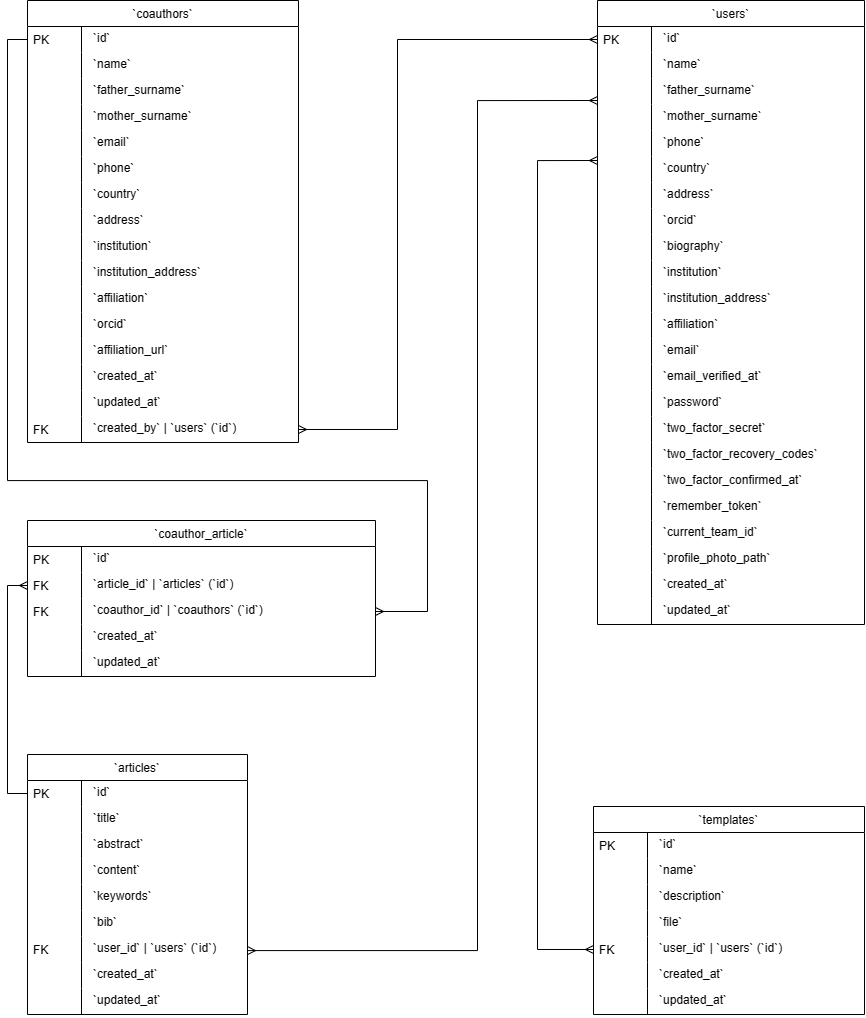
\includegraphics[width=1\textwidth]{IMAGENES/entidad-relacion.png}
    \caption{Diagrama Entidad-Relación de la Base de Datos}
\label{fig:diagrama-er}
\end{figure}

\subsection{Diccionario de Datos}
Para conocer a detalle la composición de las tablas que integran la base de datos, se desarrolló un diccionario de datos conformado por las tablas \ref{tab:users}, \ref{tab:articles}, \ref{tab:coauthors}, \ref{tab:coauthor_article}, \ref{tab:templates} donde se describe de manera específica todos los campos y tipo de dato contenidos en cada una de las tablas, a fin de entender su función.

\begin{table}[H]
    \centering
    \begin{tabular}{|p{5cm}|p{3cm}|p{1cm}|p{2cm}|p{2cm}|}
        \hline
        \textbf{Campo} & \textbf{Tipo de Dato} & \textbf{Nulo} & \textbf{Llave Primaria} & \textbf{Llave Foránea} \\
        \hline
        id & bigint UNSIGNED & No & Sí & No \\
        name & varchar(255) & No & No & No \\
        father\_surname & varchar(255) & No & No & No \\
        mother\_surname & varchar(255) & No & No & No \\
        phone & varchar(255) & No & No & No \\
        country & varchar(255) & No & No & No \\
        address & varchar(255) & Sí & No & No \\
        orcid & varchar(255) & Sí & No & No \\
        biography & text & Sí & No & No \\
        institution & varchar(255) & No & No & No \\
        institution\_address & varchar(255) & No & No & No \\
        affiliation & varchar(255) & Sí & No & No \\
        email & varchar(255) & No & No & No \\
        password & varchar(255) & No & No & No \\
        profile\_photo\_path & varchar(2048) & Sí & No & No \\
        created\_at & timestamp & Sí & No & No \\
        updated\_at & timestamp & Sí & No & No \\
        \hline
    \end{tabular}
    \caption{Tabla: users}
    \label{tab:users}
\end{table}

\begin{table}[H]
    \centering
    \begin{tabular}{|p{5cm}|p{3cm}|p{1cm}|p{2cm}|p{2cm}|}
        \hline
        \textbf{Campo} & \textbf{Tipo de Dato} & \textbf{Nulo} & \textbf{Llave Primaria} & \textbf{Llave Foránea} \\
        \hline
        id & bigint UNSIGNED & No & Sí & No \\
        title & varchar(255) & No & No & No \\
        abstract & text & Sí & No & No \\
        content & text & No & No & No \\
        keywords & text & Sí & No & No \\
        bib & text & Sí & No & No \\
        user\_id & bigint UNSIGNED & No & No & Sí \\
        created\_at & timestamp & Sí & No & No \\
        updated\_at & timestamp & Sí & No & No \\
        \hline
    \end{tabular}
    \caption{Tabla: articles}
    \label{tab:articles}

\end{table}

\begin{table}[H]
    \centering
    \begin{tabular}{|p{5cm}|p{3cm}|p{1cm}|p{2cm}|p{2cm}|}
        \hline
        \textbf{Campo} & \textbf{Tipo de Dato} & \textbf{Nulo} & \textbf{Llave Primaria} & \textbf{Llave Foránea} \\
        \hline
        id & bigint UNSIGNED & No & Sí & No \\
        name & varchar(255) & No & No & No \\
        father\_surname & varchar(255) & No & No & No \\
        mother\_surname & varchar(255) & No & No & No \\
        email & varchar(255) & No & No & No \\
        phone & varchar(255) & No & No & No \\
        country & varchar(255) & No & No & No \\
        address & varchar(255) & No & No & No \\
        institution & varchar(255) & No & No & No \\
        institution\_address & varchar(255) & No & No & No \\
        affiliation & varchar(255) & Sí & No & No \\
        orcid & varchar(255) & No & No & No \\
        affiliation\_url & varchar(255) & Sí & No & No \\
        created\_at & timestamp & Sí & No & No \\
        updated\_at & timestamp & Sí & No & No \\
        created\_by & bigint UNSIGNED & No & No & Sí \\
        \hline
    \end{tabular}
    \caption{Tabla: coauthors}
    \label{tab:coauthors}

\end{table}

\begin{table}[H]
    \centering
    \begin{tabular}{|p{5cm}|p{3cm}|p{1cm}|p{2cm}|p{2cm}|}
        \hline
        \textbf{Campo} & \textbf{Tipo de Dato} & \textbf{Nulo} & \textbf{Llave Primaria} & \textbf{Llave Foránea} \\
        \hline
        id & bigint UNSIGNED & No & Sí & No \\
        article\_id & bigint UNSIGNED & No & No & Sí \\
        coauthor\_id & bigint UNSIGNED & No & No & Sí \\
        created\_at & timestamp & Sí & No & No \\
        updated\_at & timestamp & Sí & No & No \\
        \hline
    \end{tabular}
    \caption{Tabla: coauthor\_article}
    \label{tab:coauthor_article}

\end{table}

\begin{table}[H]
    \centering
    \begin{tabular}{|p{5cm}|p{3cm}|p{1cm}|p{2cm}|p{2cm}|}
        \hline
        \textbf{Campo} & \textbf{Tipo de Dato} & \textbf{Nulo} & \textbf{Llave Primaria} & \textbf{Llave Foránea} \\
        \hline
        id & bigint UNSIGNED & No & Sí & No \\
        name & varchar(255) & No & No & No \\
        description & text & Sí & No & No \\
        file & varchar(255) & No & No & No \\
        user\_id & bigint UNSIGNED & No & No & Sí \\
        created\_at & timestamp & Sí & No & No \\
        updated\_at & timestamp & Sí & No & No \\
        \hline
    \end{tabular}
    \caption{Tabla: templates}
    \label{tab:templates}

\end{table}

\subsection{Diseño de la Interfaz de Usuario}
El diseño de la interfaz de usuario fue un aspecto importante en el desarrollo de este sistema ya que se necesitaba una interfaz amigable y responsiva que permitiera a los usuarios interactuar con el sistema de manera sencilla y eficiente. Los diseños de la interfaz de usuario se realizaron desde un inicio usando la herramienta Figma, que permite crear prototipos de alta fidelidad y realizar pruebas de usabilidad antes de empezar con el desarrollo del sistema.

Se diseñaron las interfaces de usuario para las diferentes funcionalidades del sistema, como la creación de artículos, la gestión de coautores, la subida de plantillas LaTeX, entre otras. Se crearon prototipos de alta fidelidad para algunas de las pantallas del sistema, con el objetivo de tener una guía visual para el desarrollo de la interfaz de usuario y también tener retroalimentación de los usuarios sobre el diseño de la interfaz y el flujo de interacción del sistema.

\subsubsection{Prototipos de Alta Fidelidad}
En la figura \ref{fig:prototipo-dashboard} se muestra el prototipo de alta fidelidad de la pantalla de inicio del sistema, donde los usuarios pueden ver una lista de los artículos creados y a un costado un menú de navegación con las diferentes opciones del sistema. En esta pantalla se muestra una tabla con los artículos creados por el usuario, con la opción de ver, editar y borrar cada artículo.

\begin{figure}[H]
    \centering
    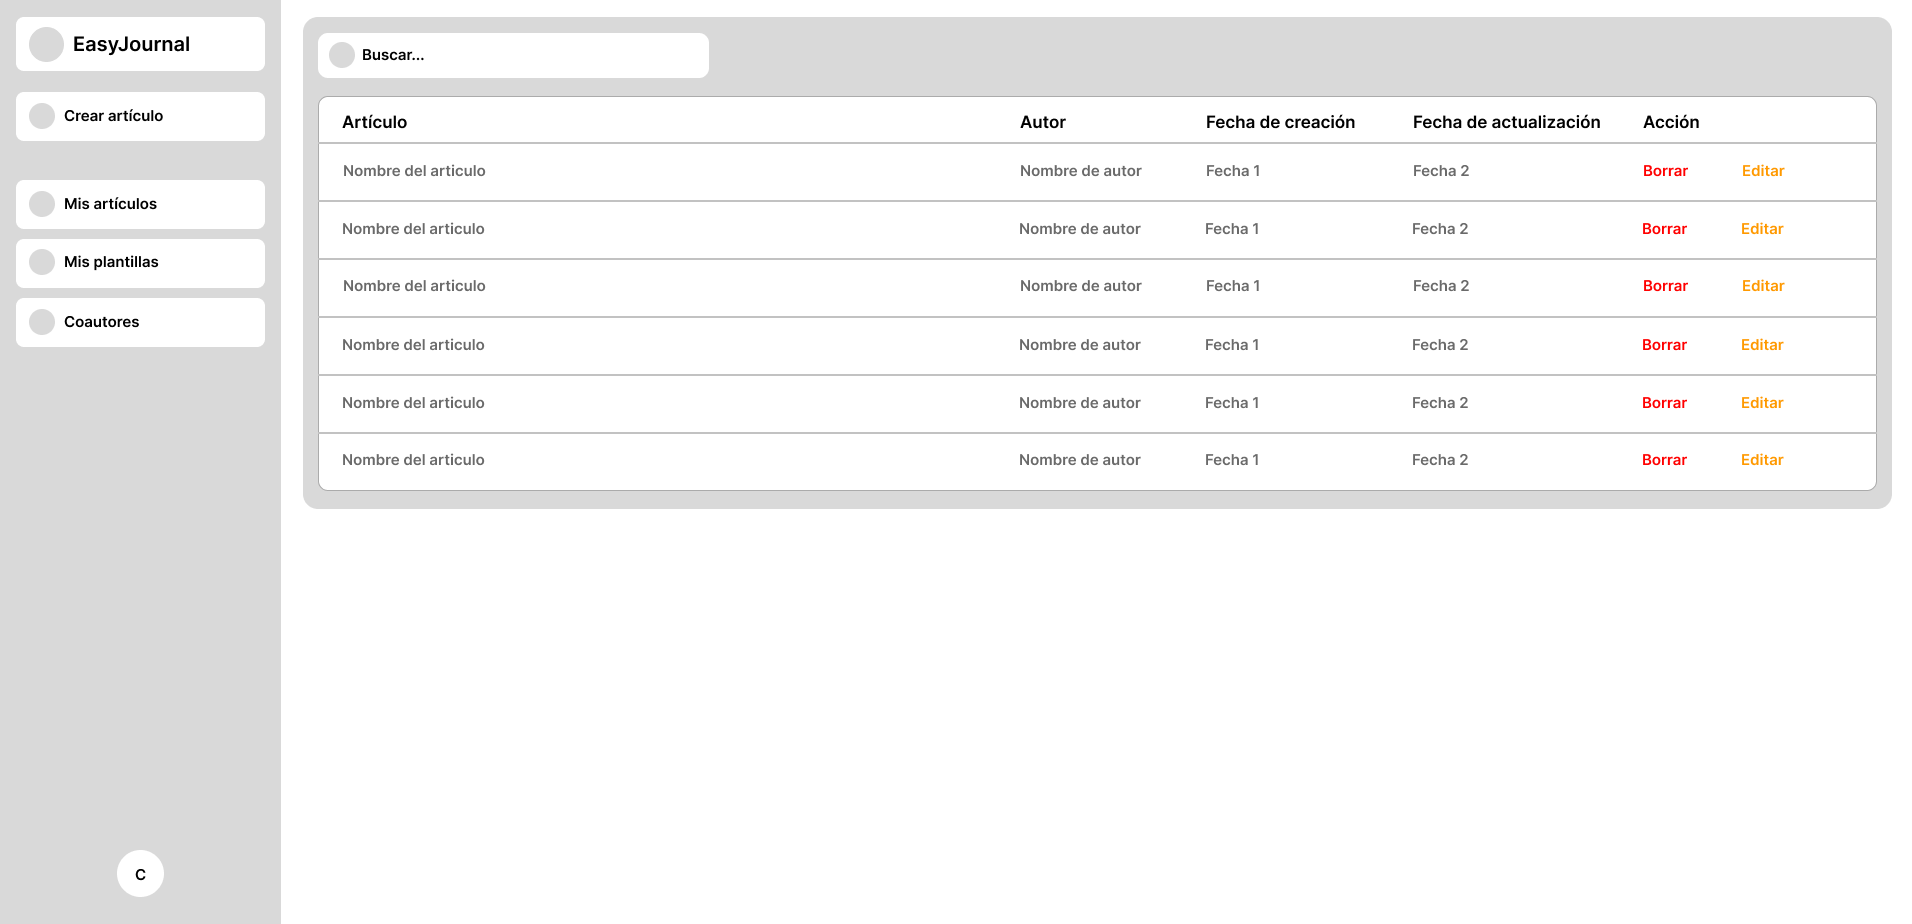
\includegraphics[width=1\textwidth]{IMAGENES/prototipo-dashboard.png}
    \caption{Prototipo de Alta Fidelidad: Pantalla de Inicio del Sistema}
\label{fig:prototipo-dashboard}

\end{figure}

En la figura \ref{fig:prototipo-crear-articulo} se muestra el prototipo de alta fidelidad de la pantalla de creación de un artículo en el sistema, donde los usuarios pueden ingresar el título del artículo y crearlo. En esta pantalla se muestra un formulario con el campo de título y un botón para guardar el artículo en el sistema.

\begin{figure}[H]
    \centering
    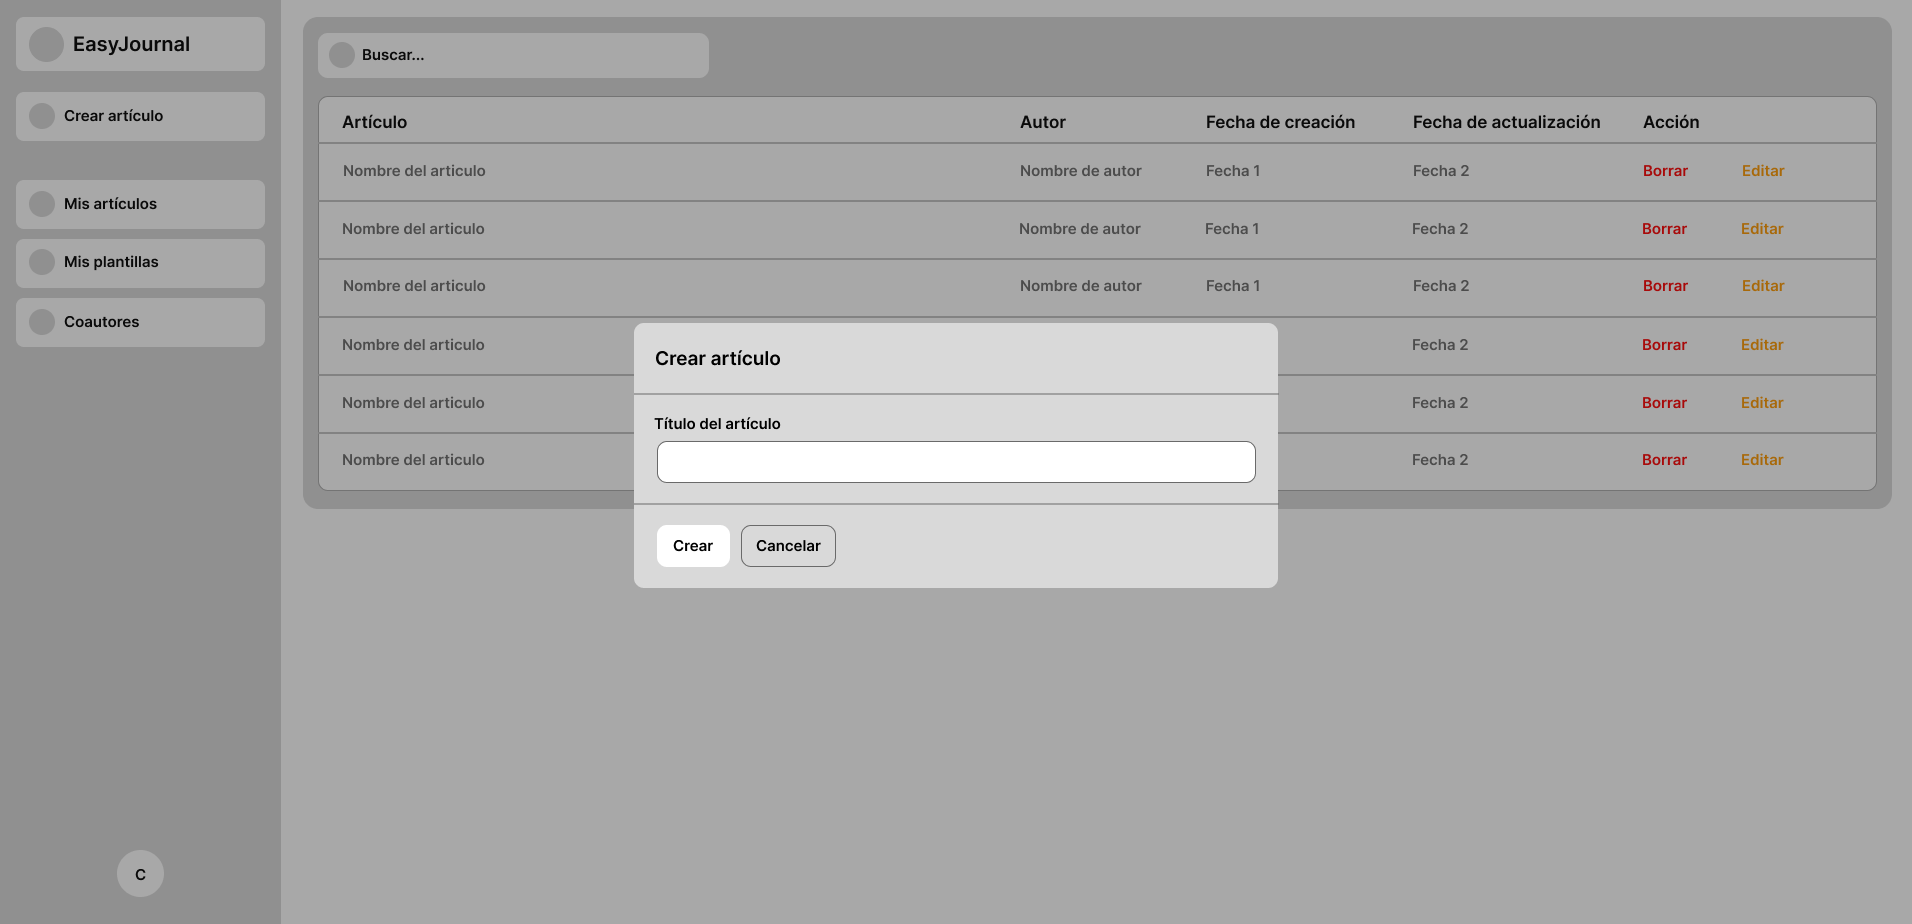
\includegraphics[width=1\textwidth]{IMAGENES/prototipo-crear-articulo.png}
    \caption{Prototipo de Alta Fidelidad: Pantalla de Creación de Artículo}
\label{fig:prototipo-crear-articulo}

\end{figure}

% En la figura \ref{fig:prototipo-crear-coautor} se muestra el prototipo de alta fidelidad de la pantalla de creación de un coautor en el sistema, donde los usuarios pueden ingresar los datos del coautor y guardarlo. En esta pantalla se muestran los campos de nombre, apellidos, correo electrónico, teléfono, país, dirección, institución, dirección de la institución, afiliación, ORCID y URL de la afiliación del coautor, y a un costado se ve una lista de los coautores creados.

% \begin{figure}[H]
%     \centering
%     \includegraphics[width=1\textwidth]{IMAGENES/prototipo-crear-coautor.png}
%     \caption{Prototipo de Alta Fidelidad: Pantalla de Creación de Coautor}
% \label{fig:prototipo-crear-coautor}

% \end{figure}


En la figura \ref{fig:prototipo-subir-plantilla} se muestra el prototipo de alta fidelidad de la pantalla de subida de una plantilla LaTeX en el sistema, donde los usuarios pueden seleccionar un archivo .zip que contenga la plantilla y subirla al sistema. En esta pantalla se muestra un formulario con el campo de archivo, nombre, descripción y un botón para subir la plantilla al sistema.

\begin{figure}[H]
    \centering
    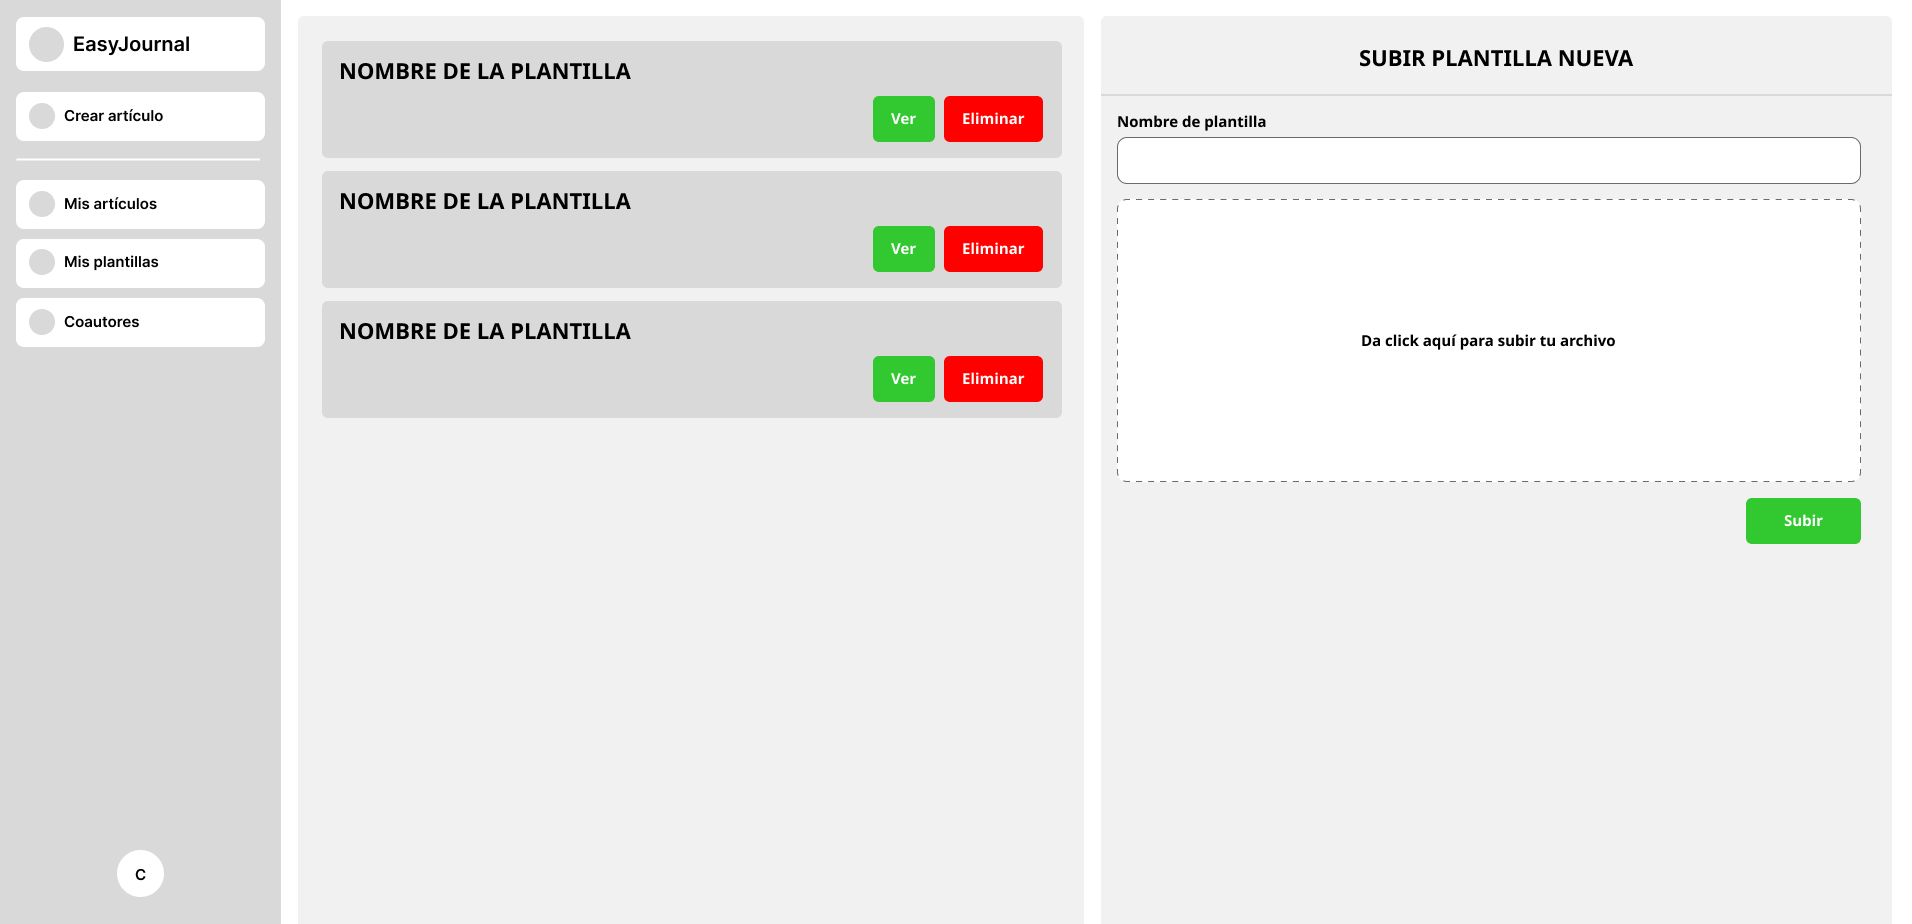
\includegraphics[width=1\textwidth]{IMAGENES/prototipo-subir-plantilla.png}
    \caption{Prototipo de Alta Fidelidad: Pantalla de Subida de Plantilla LaTeX}
\label{fig:prototipo-subir-plantilla}

\end{figure}

En la figura \ref{fig:prototipo-compilar-articulo} se muestra el prototipo de alta fidelidad de la pantalla de compilación de un artículo en una plantilla LaTeX, donde los usuarios pueden seleccionar un artículo y una plantilla para compilar el contenido del artículo en la plantilla. En esta pantalla se muestran los campos de artículo y plantilla, con la opción de compilar el artículo en la plantilla y descargar el PDF generado.

\begin{figure}[H]
    \centering
    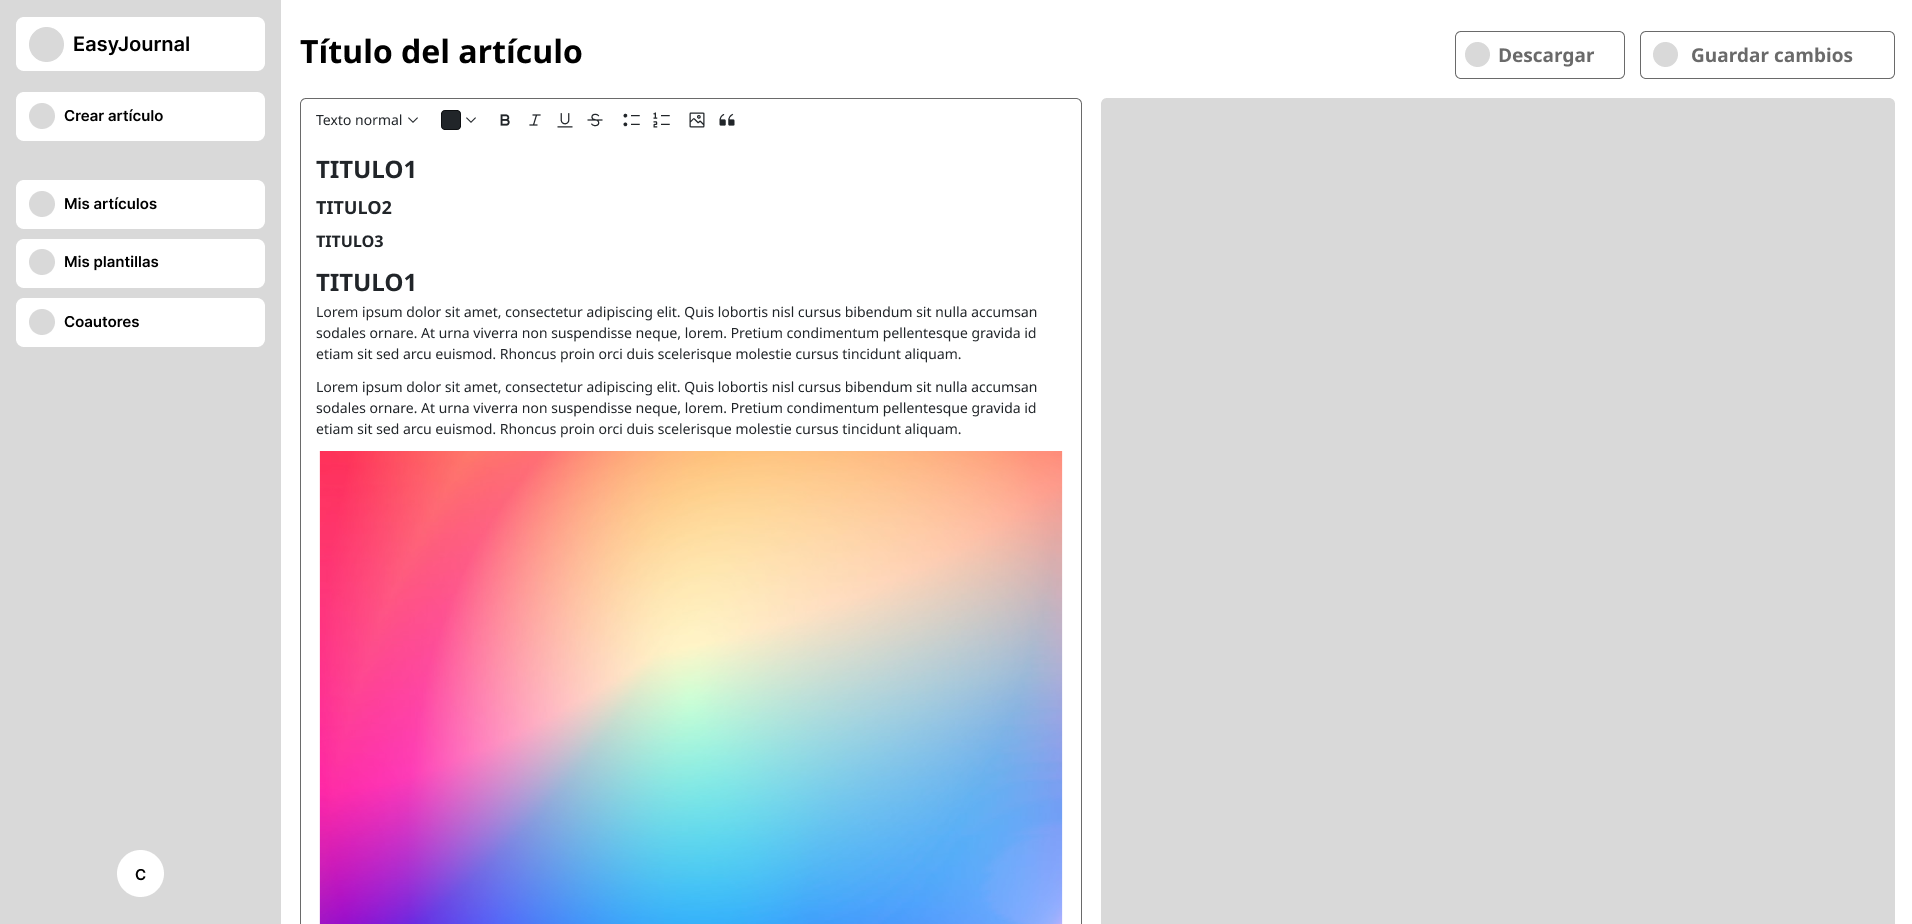
\includegraphics[width=1\textwidth]{IMAGENES/prototipo-compilar-articulo.png}
    \caption{Prototipo de Alta Fidelidad: Pantalla de Compilación de Artículo}
\label{fig:prototipo-compilar-articulo}

\end{figure}

\subsection{Desarrollo del Backend}
El desarrollo del backend del sistema se realizó utilizando el framework de php Laravel, primero se hizo la base instalando Laravel 10, luego se instaló Jetstream para manejar las sesiones, registros, recuperación de contraseñas, entre otras funcionalidades. Después de eso, se instalaron herramientas como Flowbite con Tailwind CSS, EditorJS, Symfony Process, y Gemini, se crearon migraciones, se agregaron rutas y controladores, se implementaron las funcionalidades CRUD (Crear, Leer, Actualizar, Eliminar) y se realizaron pruebas para garantizar el correcto funcionamiento del sistema. A continuación, se describe detalladamente el proceso de desarrollo del backend, incluyendo la instalación de las herramientas necesarias y la implementación de diversas funcionalidades críticas para el sistema.

\subsubsection{Instalación del Entorno de Desarrollo}
El primer paso para el desarrollo del backend fue configurar el entorno de desarrollo adecuado. Se eligió el sistema operativo Linux Mint 20.2 debido a su estabilidad y compatibilidad con las herramientas necesarias.

El proyecto comenzó con la instalación de PHP 8.2 y Composer, ya que son esenciales para el desarrollo de aplicaciones con Laravel. Una vez instaladas estas herramientas, se procedió a la instalación de Laravel 10, la última versión del framework. Posteriormente, se configuró el archivo de entorno `.env' con la información de la base de datos, datos de conexión al correo electrónico, nombre de la aplicación, llave de cifrado, entre otros parámetros importantes para el funcionamiento correcto de la aplicación.

Además, se instaló pdflatex-full junto con sus fuentes para evitar problemas al compilar plantillas que utilizan estas extensiones de LaTeX. Esta instalación fue crucial para asegurar que todos los documentos LaTeX se pudieran compilar correctamente, sin errores relacionados con fuentes o paquetes faltantes.


\subsubsection{Configuración de Jetstream}
Una vez instalado y configurado Laravel, el siguiente paso fue añadir Jetstream para gestionar la autenticación y otras funcionalidades relacionadas con los usuarios. Este paso fue de suma importancia realizarlo al inicio del proyecto antes de agregar otras funcionalidades a la aplicación, ya que Jetstream proporciona una base de archivos y rutas que facilitan la creación de un sistema de autenticación. Configurar Jetstream desde el principio evita problemas futuros al agregar funcionalidades adicionales relacionadas con los usuarios y migraciones de la base de datos.

Una vez instalado Jetstream, se configuraron las funcionalidades de usuario necesarias para el sistema desde el archivo de rutas `web.php', esto para determinar las rutas de redirección para acciones de usuario como registro e inicio de sesión, aqui se incluye un paso importante y es crear un grupo de rutas protegidas por autenticación, esto para asegurar que solo los usuarios autenticados puedan acceder a ciertas rutas. Además, se personalizaron las vistas de autenticación, incluyendo formularios de inicio de sesión y registro. Los mensajes de error y éxito mostrados al usuario tras realizar acciones también fueron ajustados.

Adicionalmente, se modificaron las migraciones de los usuarios para incluir campos adicionales relacionados con los datos de autor, como nombre, apellidos, teléfono, país, dirección, institución, dirección de la institución, biografía, ORCID, afiliación y foto de perfil. Estos campos adicionales son necesarios desde el inicio para evitar problemas al agregar funcionalidades relacionadas con los datos de autor en la aplicación. Configurar estos campos desde el principio asegura que la base de datos esté preparada para manejar toda la información requerida por el sistema sin necesidad de realizar modificaciones estructurales significativas en una etapa posterior del desarrollo.

El proceso de integración de Jetstream fue importante en el desarrollo del backend desde este momento para establecer una base sólida de gestión de usuarios, permitiendo funcionalidades avanzadas. Esta integración facilita el desarrollo de la app en gran medida ya que evita la necesidad de crear un sistema de autenticación desde cero, y permite enfocarse en la implementación de otras características del sistema.

\subsubsection{Integración de Tailwind CSS y Flowbite}
Para el diseño de la interfaz de usuario se utilizó Tailwind CSS junto con Flowbite. Esta combinación facilitó la creación de componentes reutilizables. Inicialmente, se instalaron estas dependencias mediante npm y se configuraron los archivos necesarios para incluir Tailwind CSS y Flowbite en el proyecto.

Se crearon componentes reutilizables como botones, formularios, tarjetas e inputs, utilizando las clases de Tailwind CSS, lo que resultó en un patrón de diseño personalizable y responsivo. Adicionalmente, los componentes de Flowbite como modales, tabs y dropdowns facilitaron la incorporación de elementos interactivos y dinámicos en la interfaz de usuario. Esta integración aceleró el proceso de desarrollo al proporcionar componentes listos para usar en cualquier parte de la aplicación, mejorando la coherencia, la usabilidad de la interfaz de usuario y la eficiencia con la cual se crearon las vistas.

\subsubsection{Implementación de EditorJS y Symfony Process}
Para la creación y edición de artículos científicos en formato LaTeX, se integró EditorJS ya que ofrece una interfaz intuitiva y flexible que permite a los usuarios agregar y organizar diferentes tipos de contenido, como texto, imágenes y código LaTeX embebido, de manera sencilla y eficiente.

Además, se utilizó el paquete Symfony Process para ejecutar comandos del sistema desde el código PHP, lo que facilitó la compilación de documentos LaTeX directamente desde la aplicación. El uso de Symfony Process permitío ejecutar comandos que compilan documentos LaTeX, esto da como resultado la generación de archivos PDF a partir de la plantilla que genera el sistema basado en lo que el usuario ha escrito en el editor de texto. Esto permitió a los usuarios generar documentos sin necesidad de abandonar la plataforma. 

\subsubsection{Integración de Gemini para la Gestión de Autores}
Para la edición precisa de autores en la plantilla LaTeX se usó Gemini, esta herramienta permitió mandar la seccion de autores de cualquier plantilla LaTeX junto con los datos del autor y coautores para que la API de Gemini sustituya los datos del autor en la plantilla LaTeX. La API regresa la sección con los datos ya sustituidos y listos para ser compilados.

\subsubsection{Control de Versiones con Git}
Durante el desarrollo se utilizó Github para el control de versiones del código fuente. Se crearon ramas para cada funcionalidad o tarea, lo que permitió trabajar en paralelo en diferentes partes del sistema sin interferir con el trabajo pendiente. Se realizaron commits regulares para mantener un historial de cambios. Esta práctica de control de versiones facilitó la modificación y corrección de errores en el código, y permitió trabajar de manera más eficiente en diferentes aspectos del sistema.

\subsection{Algoritmos}
A continuación se describen los algoritmos implementados en el sistema, los cuales son fundamentales para el correcto funcionamiento de la aplicación y la subida y generación de archivos LaTeX.

\subsubsection{Algoritmo de Subida de Plantilla LaTeX}
El algoritmo \ref{alg:subida-plantilla} de subida de plantilla LaTeX permite a los usuarios subir archivos .zip que contienen plantillas LaTeX a la aplicación. El algoritmo extrae los archivos del .zip, busca los archivos .tex, .cls, .bib, .bst y .sty, y los renombra para evitar conflictos de nombres. Luego, compila el archivo .tex principal y genera un archivo PDF. Finalmente, guarda la plantilla en la base de datos y muestra un mensaje de éxito o error al usuario. El algoritmo se muestra a continuación:

\begin{algorithm}
    \caption{Guardar Plantilla}
    \begin{algorithmic}[1]
    \Procedure{guardar\_plantilla}{solicitud}
        \State Validar campos requeridos en la solicitud
        \If{la validación falla}
            \State Redirigir a la página de plantillas con un mensaje de error
        \Else
            \State Guardar el archivo ZIP en la carpeta de archivos
            \State Extraer los archivos del ZIP
            \If{la extracción es exitosa}
                \State Buscar archivos .tex en la carpeta extraída
                \If{no se encuentran archivos .tex}
                    \State Redirigir a la página de plantillas con un mensaje de error
                \Else
                    \State Identificar el archivo .tex más grande
                    \State Renombrar todos los archivos en la carpeta y subcarpetas
                    \State Modificar referencias de archivos en el archivo .tex más grande
                    \State Modificar referencias de archivos en archivos .cls, .bib, .bst, .sty
                    \State Cambiar el nombre del archivo .tex más grande a \textit{main.tex}
                    \State Compilar el archivo .tex más grande
                    \If{se genera el archivo PDF}
                        \State Crear y almacenar un objeto Template en la base de datos
                        \State Crear un nuevo archivo ZIP con los archivos modificados
                        \State Redirigir a la página de plantillas con un mensaje de éxito
                    \Else
                        \State Mostrar un mensaje de error
                        \State Eliminar el archivo ZIP y la carpeta extraída
                        \State Redirigir a la página de plantillas
                    \EndIf
                \EndIf
            \EndIf
        \EndIf
    \EndProcedure
    \end{algorithmic}
    \caption{Algoritmo de Subida de Plantilla LaTeX}
    \label{alg:subida-plantilla}
\end{algorithm}

\subsubsection{Algoritmo de Previsualización de Plantilla LaTeX}
El algoritmo \ref{alg:previsualizacion-plantilla} de previsualización de plantilla LaTeX permite a los usuarios ver una vista previa del archivo PDF generado a partir de la plantilla LaTeX. El algoritmo compila el archivo .tex principal y genera un archivo PDF, luego mueve el archivo PDF al directorio público y devuelve la URL del archivo PDF para mostrarlo en la vista. El algoritmo se muestra a continuación:

\begin{algorithm}
    \caption{Previsualizar Plantilla}
    \begin{algorithmic}[1]
    \Procedure{previsualizar\_plantilla}{plantilla}
        \State Definir la ruta donde se extraen los archivos basada en la plantilla
        \State Definir la ruta del archivo principal .tex
        \State Crear un script bash para compilar el archivo .tex y generar el PDF
        \State Guardar el script en un archivo .sh
        \State Ejecutar el script utilizando el comando Process de Symfony
        \State Definir la ruta del archivo PDF generado
        \State Obtener el nombre del archivo PDF
        \If{la carpeta "pdfs" no existe}
            \State Crearla
        \Else
            \State Borrar todos los archivos dentro de la carpeta "pdfs"
        \EndIf
        \State Mover el archivo PDF al directorio público en la carpeta "pdfs"
        \State Obtener la URL del archivo PDF
        \State Devolver la vista de previsualización con la URL del PDF
    \EndProcedure
    \end{algorithmic}
    \caption{Algoritmo de Previsualización de Plantilla LaTeX}
    \label{alg:previsualizacion-plantilla}
\end{algorithm}

\subsubsection{Algoritmo de Compilación de Artículo Generado}

El algoritmo \ref{alg:compilacion-articulo} de compilación de artículo generado permite a los usuarios compilar un artículo en una plantilla LaTeX seleccionada. El algoritmo sustituye los datos del autor y coautores en la plantilla LaTeX, compila el archivo .tex y genera un archivo PDF. Finalmente, guarda el archivo PDF en el directorio público y devuelve la URL del archivo PDF para mostrarlo en la vista. El algoritmo se muestra a continuación:

\begin{algorithm}
    \caption{Compilar Artículo Generado}
    \begin{algorithmic}[1]
    \Procedure{compilar\_articulo}{articulo}
        \State Validar los datos del formulario
        \State Actualizar los campos del artículo
        \State Definir funciones para quitar comentarios, abstract, keywords, contenido del archivo .tex
        \State Definir función para enviar el archivo .tex a Gemini
        \State Definir funciones para reemplazar contenido, abstract y keywords en el archivo .tex
        \State Definir función para agregar paquetes necesarios al archivo .tex
        \State Definir funciones para generar listas, imágenes y tablas en LaTeX
        \State Obtener el contenido del artículo
        \State Generar el contenido LaTeX del artículo
        \If{no se selecciona una plantilla}
            \State Crear el archivo .tex con el contenido del artículo
            \State Compilar el archivo .tex
            \If{se genera el archivo PDF}
                \State Redirigir a la vista de edición del artículo con la URL del PDF
            \Else
                \State Mostrar un mensaje de error
                \State Redirigir a la vista de edición del artículo
            \EndIf
        \Else
            \State Obtener la plantilla seleccionada
            \State Extraer los archivos de la plantilla
            \State Eliminar archivos innecesarios de la plantilla
            \State Renombrar el archivo .tex principal
            \State Generar el contenido LaTeX del artículo
            \State Crear el archivo .tex con el contenido del artículo
            \State Definir funciones para quitar comentarios, abstract, keywords, contenido del archivo .tex
            \State Enviar el archivo .tex a Gemini
            \State Agregar paquetes necesarios al archivo .tex
            \State Reemplazar contenido, abstract y keywords en el archivo .tex
            \State Compilar el archivo .tex
            \If{se genera el archivo PDF}
                \State Redirigir a la vista de edición del artículo con la URL del PDF
            \Else
                \State Mostrar un mensaje de error
                \State Redirigir a la vista de edición del artículo
            \EndIf
        \EndIf
    \EndProcedure
    \end{algorithmic}
    \label{alg:compilacion-articulo}
\end{algorithm}

\subsubsection{Algoritmo para descargar un artículo en formato PDF}
El siguiente algoritmo \ref{alg:descargar-pdf} describe el proceso de descarga de un artículo en formato PDF. Una vez que el artículo ha sido compilado con éxito, se puede descargar en formato PDF.

\begin{algorithm}
    \caption{Descargar Artículo en PDF}
    \begin{algorithmic}[1]
    \Procedure{descargar\_pdf}{articulo}
        \State Descargar el archivo PDF del artículo
        \State Retornar la respuesta de descarga
    \EndProcedure
    \end{algorithmic}
    \label{alg:descargar-pdf}
\end{algorithm}

\subsubsection{Algoritmo para descargar un artículo en formato ZIP}
El siguiente algoritmo \ref{alg:descargar-zip} describe el proceso de descarga de un artículo en formato ZIP. Una vez que el artículo ha sido compilado con éxito, se puede descargar en formato ZIP.

\begin{algorithm}
    \caption{Descargar Artículo en ZIP}
    \begin{algorithmic}[1]
    \Procedure{descargar\_zip}{articulo}
        \State Crear la carpeta \textit{templates\_zip} si no existe
        \State Borrar el contenido de la carpeta \textit{templates\_zip}
        \State Crear el archivo ZIP del artículo
        \State Descargar el archivo ZIP del artículo
        \State Retornar la respuesta de descarga
    \EndProcedure
    \end{algorithmic}
    \label{alg:descargar-zip}
\end{algorithm}

